\chapter[Organização Github]{Organização Github}

\section{Visão Geral}
A organização do Agromart no Github foi criada no ano de 2021, ela foi utilizada para o desenvolvimento do Agromart ao longo de três trabalhos de conclusão de curso, durante esses trabalhos foram criados 7 repositórios. Repositórios do aplicativo móvel, API Dicionário, API principal, Frontend Web, que foi arquivado, dois repositórios de documentação e um repositório ".github" que insere a descrição da organização. 

Ao longo dos diferentes trabalhos desenvolvidos, algumas funcionalidades foram descontinuadas, \textit{branches} foram deixadas em aberto e não foram mescladas totalmente. Iremos focar esse trabalho nos três repositórios de código fonte utilizados pelo Agromart hoje, o da API dicionário, da API principal e do aplicativo móvel. Diante dessa situação surge a necessidade de analisar o que cada um desses repositórios e ramos de desenvolvimento contém, para sintetizar todo o trabalho feito de uma forma organizada para dar unidade ao Agromart e facilitar os futuros desenvolvimentos.

\section{Mapeamento de \textit{branches} e unificação}
Essa seção busca trazer mais informações sobre as \textit{branches} que existiam e cada repositório e qual seu conteúdo, bem como os resultados obtidos com a unificação delas na \textit{branch} "devel". Como a API dicionário não possui mais de uma \textit{branch}, ela não será abordada nessa seção.

\subsection{Aplicativo móvel}
O repositório do aplicativo móvel do Agromart se chama "mobile-client" e inicialmente possui quatro \textit{branches} ativas. As \textit{branches} ativas eram: "devel", "tcc-abner-rafael", "csa\_choose", "csa\_page\_test", "feature/US03-realizar-pagamento" e "master".

\begin{figure}[h]
	\centering
	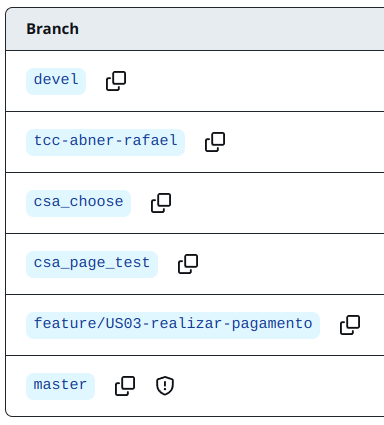
\includegraphics[keepaspectratio=true,scale=0.5]{figuras/banches_mobile.png}
	\caption{Branches repositório do aplicativo móvel}
\end{figure}

Na \textit{branch} "tcc-abner-rafael", haviam algumas alterações, como atualização parcial da versão da SDK do Expo e algumas correções de erros em tempo de execução na tela de login.

Na \textit{branch} "csa\_page\_test", havia a criação de um novo componente de seleção de CSA>

Na \textit{branch} "csa\_choose", haviam alterações da pastas \textit{android} e \textit{ios}, bem como alterações na seleção da url base através da API dicionário, todas alterações da \textit{branch} "csa\_page\_test" também estão presentes nessa.

A \textit{branch} "feature/US03-realizar-pagamento", já estava totalmente mergeada em "devel" e podia ser excluida de forma segura.

\subsection{API principal}
O repositório da API principal do Agromart se chama "api" e inicialmente estava com 4 \textit{branches} ativas. As \textit{branches} ativas eram: "devel", "tcc-abner-rafael", "automate-deploy" e "master".

\begin{figure}[h]
	\centering
	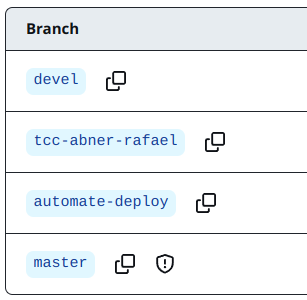
\includegraphics[keepaspectratio=true,scale=0.5]{figuras/branches_api.png}
	\caption{Branches repositório da API principal}
\end{figure}

As \textit{branches} "devel" e "master" são respectivamente as \textit{branches} de desenvolvimento e principal

O código unificado dessas \textit{branches} foram incorporadas à \textit{branch} de desenvolvimento, e neste repositório foram mantidas apenas as "devel" e "master".

A \textit{branch} "automate-deploy" é onde foi desenvolvida a automatização de publicação, ela já estava com sua funcionalidade principal incorporada na "devel", tendo como diferença apenas alterações relacionados a variáveis de ambiente. 

A branch "tcc-abner-rafael" possuía algumas correções de erros da API principal.


\subsection{Repositório API Dicionário}
O repositório da API Dicionário do Agromart se chama "api-dicionario" e continha apenas uma \textit{branch} "main". Dessa forma, não foi necessário nenhum trabalho de análise e unificação de \textit{branches}.

\begin{figure}[h]
	\centering
	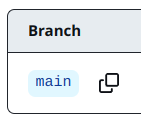
\includegraphics[keepaspectratio=true,scale=0.5]{figuras/branches_api_dicionario.png}
	\caption{\textit{Branches} Repositório API Dicionário}
\end{figure}


\subsection{Resultados}

Após o mapeamento do que havia em cada \textit{branch} e o entendimento de que eles possuíam códigos úteis, todas as \textit{branches} foram mescladas em "devel" sem nenhum conflito, e a partir da \textit{branch} de desenvolvimento, tanto no repositório do aplicativo quanto no repositório da API principal, iniciamos então a próxima etapa do trabalho, que seria correção de defeitos até chegar em um MVP estável.

Ao final dos \textit{merges}, como vemos na Fig. \ref{branches_after}, ambos repositórios ficaram apenas com duas \textit{branches}, "devel" e "master", que serão o ponto de partida para o desenvolvimento das correções. Além disso, após todas as correções feitas e conclusão do trabalho, a \textit{branch} "master" foi atualizada com o conteúdo de "devel".

\begin{figure}[h]
	\centering
	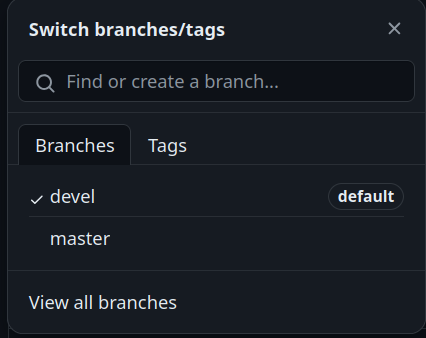
\includegraphics[keepaspectratio=true,scale=0.5]{figuras/branches-after.png}
	\caption{Resultado após unificação}
 	\label{branches_after}
\end{figure}